\documentclass{article}

\usepackage{amsmath}
\usepackage{amsfonts} % For math fonts.
\usepackage{amssymb} % For other math symbols not covered by amsmath.
\usepackage[pdftex]{graphicx} % For pictures, use \includegraphics[scale=decimal]{pic.png}; must be a .png file type.
\usepackage{multicol}
\usepackage{textcomp}
\usepackage[colorlinks = true, urlcolor = blue]{hyperref}
\usepackage{enumitem}
\usepackage{graphbox} 
\usepackage{subfig}
\usepackage{multicol}
\usepackage{nopageno}
\usepackage{bm}


\usepackage{tikz}
\usetikzlibrary{positioning, calc}
\usetikzlibrary{shapes.geometric,angles,quotes}
\usepackage{tikz-3dplot}


%page formatting
\usepackage{fullpage}
\setlength{\parindent}{0pt}


\newcommand{\tab}{\hspace*{0.25in}}
\newcommand{\csq}[1]{\reflectbox{''}#1''}  %This produces CS style quotes.
\newcommand{\csqt}[1]{\text{\reflectbox{''}#1''}}  %This produces CS style quotes as text.


\usepackage{listings}
\lstset
{ %Formatting for code in appendix
    language=Python,
    basicstyle=\footnotesize,
    numbers=left,
    stepnumber=1,
    showstringspaces=false,
    tabsize=2,
    breaklines=true,
    breakatwhitespace=false,
}


\begin{document}



%split_point

%\end{document}
Lone Star \hfill Files quiz\\
section 4\\
\begin{enumerate}
\item (14.1) 
		Write 100 integers created randomly into a file named \textit{QuizInts.txt}. 
		The numbers should be between 50 and 200 (inclusively). 
		Each number should be on a new line.\\
		Hint: Your code will likely use the following two lines of code somewhere in your program.\\
			\tab import random.\\
			\tab random.randint(50,200)

\item (14.2) 
		A local gym keeps a log of how many calories were burned in workout sessions each day, stored in a file called \textit{CaloriesBurnedData.txt}.  
		Each line of the file includes the date and the total number of calories burned by all gym members on that day.  
		A portion of the file is shown below.  
		Write a program that reads the file and prints the day with the highest number of calories burned.
		
		\begin{flushright}
			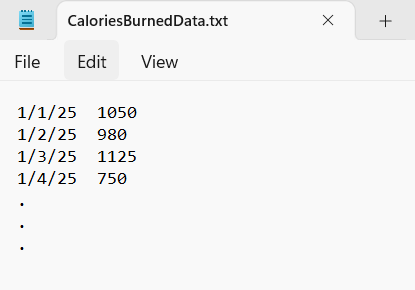
\includegraphics[scale=.65]{imgs/CaloriesBurnedData.PNG}
		\end{flushright}


\item (14.3) 
		Create a python program that writes the name and age of everyone in your family to .csv file.
		There should be a column for the name with a header titled Name, and there should be a column 
		for the age with a header titled Age.
		Do not use the csv module. You may make up fake family members if you choose. The result
		should look similar to the following.
		
		\begin{flushright}
			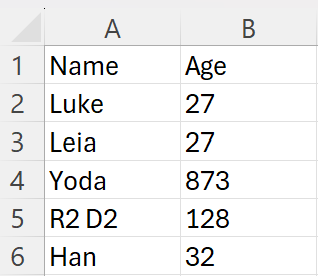
\includegraphics[scale=.65]{imgs/WritingFamily.PNG}
		\end{flushright}



%Write a few that write to write with multiple columns using a clear delimeter. 



%end_of_questions
%make sure to leave at least one blank line below

\end{enumerate}
\pagebreak
Dot Matrix \hfill Files quiz\\
section 5\\
\begin{enumerate}
\item (14.1)
		Create a file named \textit{MyName.txt}, and write your name to it (your actual name).	 
		Then read the file and print the letters of your name one at a time where each letter is on a new line.
		\begin{figure}[ht]
			\centering
			\begin{minipage}[b]{.4\textwidth}
				\centering
				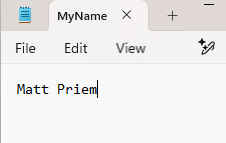
\includegraphics[scale=1]{imgs/nameFile.png}
				\caption{This is the file.}	
			\end{minipage}
			\hspace*{2em}
			\begin{minipage}[b]{.4\textwidth}
				\centering
				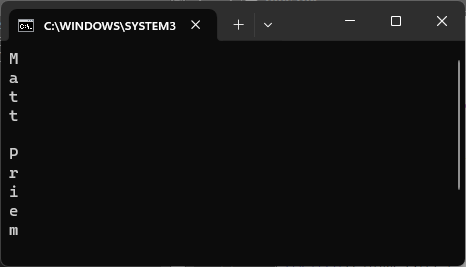
\includegraphics[width=1\textwidth]{imgs/nameOutput.png}
				\caption{This is the output.}
			\end{minipage}
		\end{figure}


\item (14.2) 
		A city library keeps track of the number of visitors each day in a file named 
		\textit{LibraryVisitsData.csv}.  
		The file contains a date and the number of visitors who entered the library on that date.  
		There is one entry for each day of the year. A portion of that file is shown below.  
		Write a program that reads the file, calculates, and prints the average number of visitors 
		per day over the year.
		
		\begin{flushright}
			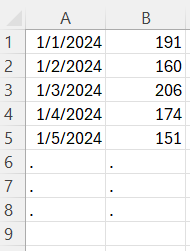
\includegraphics[scale=.65]{imgs/LibraryVisitsData.PNG}
		\end{flushright}


\item (14.3) 
		Create a python program that writes the name and age of everyone in your family to .csv file.
		There should be a column for the name with a header titled Name, and there should be a column 
		for the age with a header titled Age.
		Do not use the csv module. You may make up fake family members if you choose. The result
		should look similar to the following.
		
		\begin{flushright}
			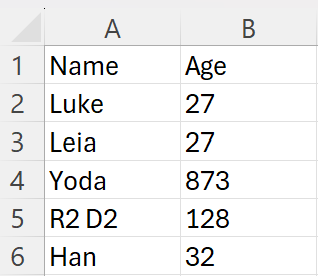
\includegraphics[scale=.65]{imgs/WritingFamily.PNG}
		\end{flushright}



%Write a few that write to write with multiple columns using a clear delimeter. 



%end_of_questions
%make sure to leave at least one blank line below

\end{enumerate}
\pagebreak
Dark Helmet \hfill Files quiz\\
section 4\\
\begin{enumerate}
\item (14.1)
		Assume you have a text file called \textit{aMorePerfectUnion.txt} that contains a transcript 
		of Barack Obama's March $18^{th}$, 2008 speech \textit{A More Perfect Union}. Create a 
		dictionary consisting each word and the amount of times that word appears in the speech. 
		Print the dictionary.

%end_of_questions
%make sure to leave at least one blank line below

\item (14.2) 
		A local middle school is trying to count the total number of lunches they served last year.  
		They have a text file named \textit{LunchData.txt} that has a date and the number of lunches served on that date.    
		There is one entry for every day last year.  A portion of that file is displayed below.  
		Write a program that calculates and then prints the total number of lunches served last year. 
		\begin{flushright}
			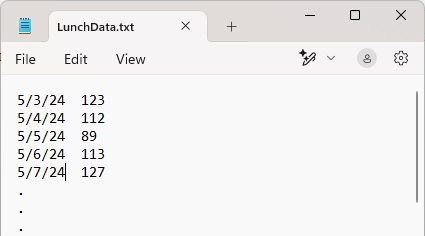
\includegraphics[scale=.65]{imgs/LunchData.PNG}
		\end{flushright}




\item (14.3) 
		Create a python program that writes the name and age of everyone in your family to .csv file.
		There should be a column for the name with a header titled Name, and there should be a column 
		for the age with a header titled Age.
		Do not use the csv module. You may make up fake family members if you choose. The result
		should look similar to the following.
		
		\begin{flushright}
			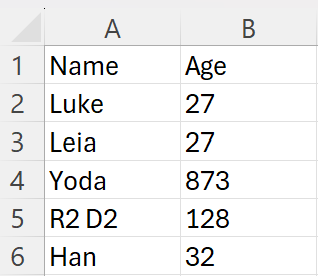
\includegraphics[scale=.65]{imgs/WritingFamily.PNG}
		\end{flushright}



%Write a few that write to write with multiple columns using a clear delimeter. 



%end_of_questions
%make sure to leave at least one blank line below

\end{enumerate}
\pagebreak
President Skroob \hfill Files quiz\\
section 1\\
\begin{enumerate}
\item (14.1) 
		Write a Python program that will open a file named \textit{thisFile.txt} and write every 
		other line into the file
		\textit{thatFile.txt}

\item (14.2) 
		A city library keeps track of the number of visitors each day in a file named 
		\textit{LibraryVisitsData.csv}.  
		The file contains a date and the number of visitors who entered the library on that date.  
		There is one entry for each day of the year. A portion of that file is shown below.  
		Write a program that reads the file, calculates, and prints the average number of visitors 
		per day over the year.
		
		\begin{flushright}
			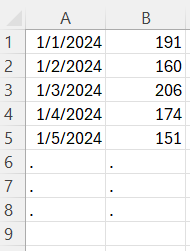
\includegraphics[scale=.65]{imgs/LibraryVisitsData.PNG}
		\end{flushright}


\item (14.3) 
		Create a python program that writes the name and age of everyone in your family to .csv file.
		There should be a column for the name with a header titled Name, and there should be a column 
		for the age with a header titled Age.
		Do not use the csv module. You may make up fake family members if you choose. The result
		should look similar to the following.
		
		\begin{flushright}
			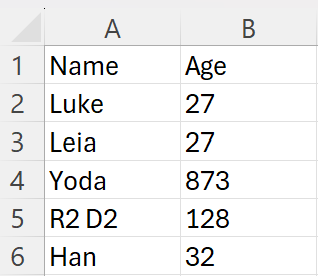
\includegraphics[scale=.65]{imgs/WritingFamily.PNG}
		\end{flushright}



%Write a few that write to write with multiple columns using a clear delimeter. 



%end_of_questions
%make sure to leave at least one blank line below

\end{enumerate}
\pagebreak
\end{document}